\section{ Methods}
\label{sect:prelim}

The following experiment compare XTREE and BELLTREE against  
Alves, Shatnawi, Oliveira et al.  




\subsection{A Strategy for Evaluating Planners}

It can be somewhat difficult to judge the effects of applying plans
to software projects. These plans cannot be assessed just by a rerun of the test suite for three reasons: (1) The defects were recorded by a post release bug tracking system. It is entirely possible it escaped detection by the existing test suite; (2) Rewriting test cases to enable coverage of all possible scenarios presents a significant challenge; and (3) It may take a significant amount of effort to write new test cases that identify these changes as they are made.

To resolve this problem, SE researchers such as
Cheng et al.~\citep{Cheng10}, O'Keefe et al.~\citep{OKeeffe08, OKeeffe07}, 
Moghadam~\citep{Moghadam2011} and Mkaouer et al.~\citep{Mkaouer14}
use a {\em verification oracle} learned separately from the primary oracle. This oracles assesses how defective the code is before and after some code changes. For their oracle, Cheng, O'Keefe, Moghadam and Mkaouer et al. use the QMOOD quality model~\citep{Bansiya02}. A shortcoming of QMOOD is that quality models learned from other projects may perform poorly when applied to new projects~\citep{localvsglobal}. As a results, we eschew using these methods in favor of evaluation strategies discussed in the rest of this section.

% As an example, consider \fig{overlap_example}; there we have 2 sets of changes: (1) Changes made by developers ($\mathcal{D}$), and (2) Changes recommended by the planner ($\mathcal{P}$). In each case we have 3 possible actions for every metric: (1) Make no change (`$\cdot$'), (2) Increase (`$+$'), and (3) Decrease (`$-$'). The intersection of the changes represents the number of times the actions taken by the developers is the same as the actions recommended by the planner. This the above example, the intersection, $\mathcal{D}\cap\mathcal{P}=7$, out of a total of $\mathcal{D}\cup\mathcal{P}=9$ possible actions. This leads to $Overlap=\frac{7}{9}\times100=77.77\%$.

\subsubsection{The \ktest}
\label{sect:ktest}

This section offers details on the evaluation method introduced
at the end of \tion{hoc}.

In order to measure the extent to which the recommendations made by planning tools matches those undertaken by the developers,
we assess the impact making those changes would have on an upcoming release of a project. For this purpose, we propose the \ktest. 

\respto{2-A}~{\color{steel}We say that a project $\mathcal{P}$ is released in versions $\mathcal{V}\in\{\mathcal{V}_{i}, \mathcal{V}_j, \mathcal{V}_{k}\}$. Here, in terms of release dates, $\mathcal{V}_i$ precedes $\mathcal{V}_j$, which in turn precedes $\mathcal{V}_k$.} We will use these three sets for  \textit{train}, \textit{test}, and \textit{validation}, respectively\footnote{And recall in 
\tion{hoc} these versions were  given less formal names, specifically
{\em older, newer, latest}.}. These
three sets  are used as follows:

\be
\item First, train the planner on version $\mathcal{V}_{i}$. Note: this could either be data that is either from a previous release, or it could be data from the bellwether project. 

\item Next, use the planner to generate plans to reduce defects for files that were reported to be buggy in version $\mathcal{V}_{j}$.

\item Finally, on version $\mathcal{V}_{k}$, for \textit{only} the files that were reported to be buggy in the previous release, we measure the OO metrics. 
\ee

Having obtained the changes at version $\mathcal{V}_{k}$ we can now (a) measure the \textit{overlap} between plans recommended by the planner and the developer's actions, and (b) count the number of defects reduced (or possibly increased) when compared to the previous release. Using these two measures, we can assess the impact of implementing these plans. Details on measuring each of these are discussed in the subsequent parts of this section.

To compute that overlap, we proceeded as follows.
Consider  two sets of changes: 
\be
\item
$\mathcal{D}$: The changes that developers made, perhaps in response to the issues raised in a post-release issue tracking system; 
\item
$\mathcal{P}$: The plans recommended by an automated planning tool, \textit{overlap} attempts to compute the extent to which a developer's action matches that of the actions recommended by planners. 
\ee
To measure this \textit{overlap}, we use Jaccard similarity:
\begin{equation}
\setlength{\abovedisplayskip}{0pt}
\setlength{\belowdisplayskip}{0pt}
\label{eq:jaccard}
\mathit{Overlap} = \frac{|\mathcal{D} \cap \mathcal{P}|}{|\mathcal{D} \cup \mathcal{P}|}\times 100  
\end{equation}
\begin{figure}[pt!]
    \centering
    \resizebox{\linewidth}{!}{
    \begin{tabular}{c|ccccccccc}
    & DIT & NOC & CBO & RFC & FOUT & WMC & NOM & LOC & LCOM \bigstrut\\\hline
    Version $\mathcal{V}_{k}$ & 3 & 4 & 4 & 2 & 5 & 2.5 & 3 & 400 & 6 \bigstrut\\
    $\mathcal{P}\rightarrow\mathcal{V}_{k+1}$ & \cellcolor[HTML]{D0D0D0}$\cdot$ & \cellcolor[HTML]{D0D0D0}$\cdot$ & $\cdot$  & \cellcolor[HTML]{D0D0D0}$[4,7]$  & $\cdot$   & \cellcolor[HTML]{D0D0D0}$[3,6]$  & \cellcolor[HTML]{D0D0D0}$[4,7]$  & \cellcolor[HTML]{D0D0D0}$[1000, 2000]$  & \cellcolor[HTML]{D0D0D0}$[1,4]$  \bigstrut\\
    $\mathcal{D}\rightarrow\mathcal{V}_{k+1}$ & \cellcolor[HTML]{D0D0D0}$3$ & \cellcolor[HTML]{D0D0D0}$4$ & $3$  & \cellcolor[HTML]{D0D0D0}$5$  & $3$   & \cellcolor[HTML]{D0D0D0}$5$  & \cellcolor[HTML]{D0D0D0}$4$  & \cellcolor[HTML]{D0D0D0}$1500$  & \cellcolor[HTML]{D0D0D0}$2$  \\
    \end{tabular}}
    \begin{equation*}
        \setlength{\abovedisplayskip}{0em}
        \setlength{\belowdisplayskip}{-1.1em}
        Overlap = \frac{|\mathcal{D} \cap \mathcal{P}|}{|\mathcal{D} \cup \mathcal{P}|}\times 100 = \frac{7}{9}\times100 = 77.77\%
    \end{equation*}
    \caption{A simple example of computing overlap. Here a `$\cdot$' represents \textit{no-change}. Columns shaded in \colorbox{lightgray}{gray} indicate a match between developer's changes and planner's recommendations.}
    \label{fig:overlap_example}
    \end{figure}    
In other words, we measure the ratio of the size of the intersection between the developers plans and the size of all possible \textit{changes}.  Note
that  the {\em larger} the intersection between the changes made by the developers to the changes recommended by the planner, then the {\em greater} the overlap. 

An simple example of how overlap is computed is illustrated in~\fig{overlap_example}. Here, we have 9 metrics and let's say a defective file version $\mathcal{V}_{k}$ has metric values corresponding to row labeled Version $\mathcal{V}_{k}$. The row labeled $\mathcal{P}\rightarrow\mathcal{V}_{k+1}$ contains set of treatments recommended by a planner $\mathcal{P}$ for version $\mathcal{V}_{k+1}$ (note that the recommendations are ranges of values rather than actual numbers). Finally, the row labeled $\mathcal{D}\rightarrow\mathcal{V}_{k+1}$ are the result of a developer taking certain steps to possibly reduce the defects in the file for version $\mathcal{V}_{k+1}$. We see that in two cases (CBO and FOUT) the developers actions led to changes in metrics that were not prescribed by the planner. But in 7 cases, the developers actions matched the changes prescribed by the planner. Computing overlap as per~\eq{jaccard}, produces an overlap value of $77\%$.
%Note again, that we only ever measure overlap on \textit{defective} files in version $\mathcal{V}_{k}$ that were defective. There may be several files in $\mathcal{V}_{k}$ that are not defective. These non-defective files are ignored so as not bias our findings.

\subsection{Presentation of Results}

Using the {\ktest}  and overlap counts defined above,
we can measure  the overlap between the planners' recommendations and developers actions. With this, plot three kinds of charts to discuss our results:
\begin{figure}[t!]
\small
\centering
\begin{tabular}{|p{0.95\linewidth}|} \hline
%\vspace{0.02cm}
%\textbf{Planner Effectiveness Curve:}
%\textbf{Defect Decreased (Increased) vs. Overlap Curve}
\begin{center}
    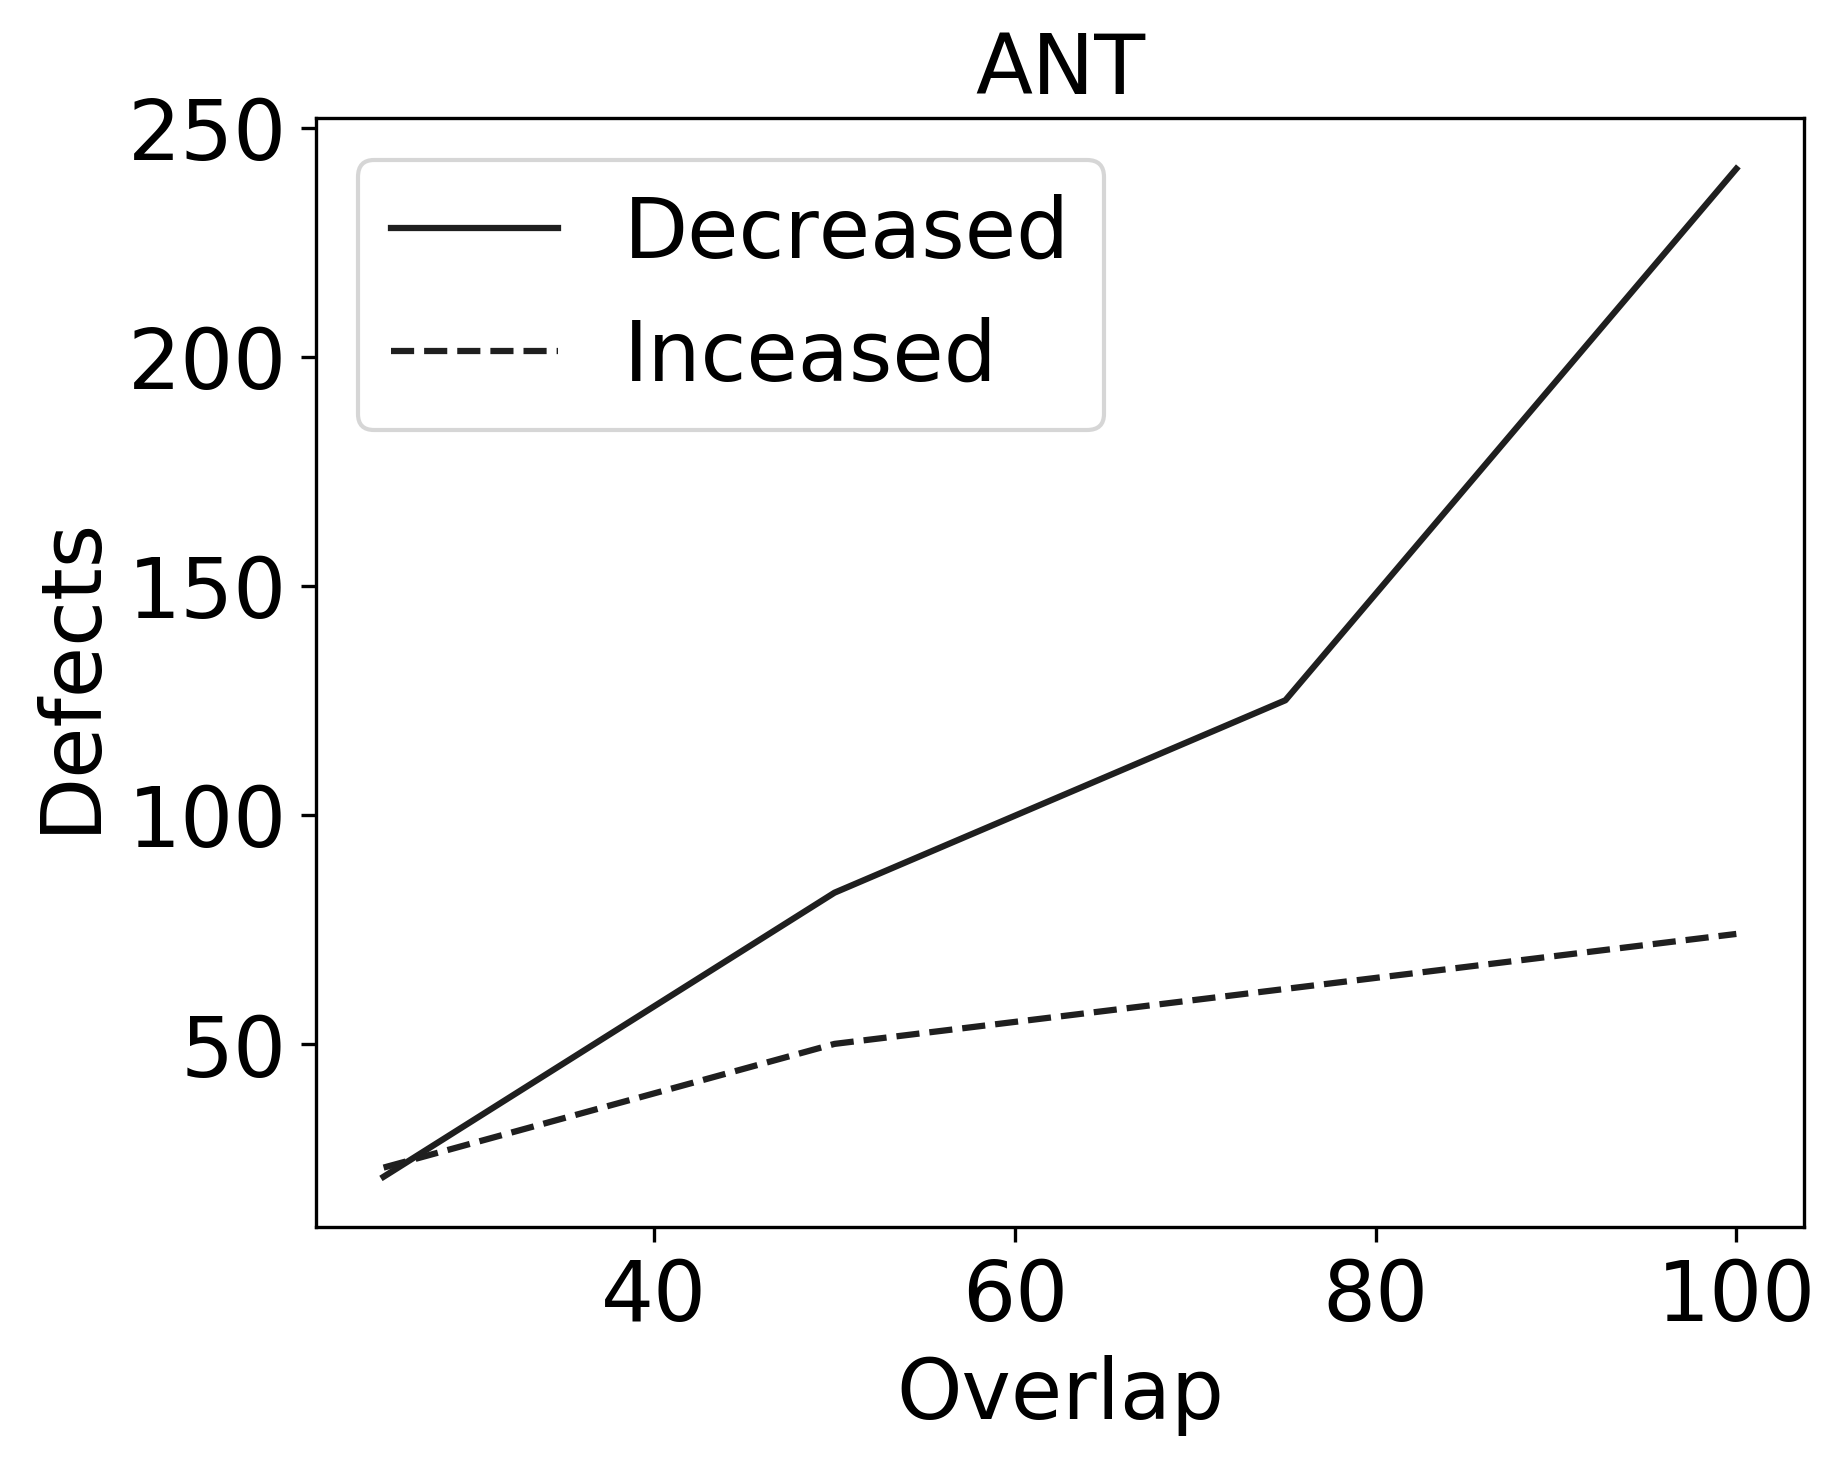
\includegraphics[width=0.7\linewidth]{sample_ant.png}
\end{center}
\[
\mathit{AUPEC} = \int_{0}^{1} f(x) \, dx \hfill
\]
\[\approx \tfrac{\Delta x}{3}\left(f(x_0) + 4f(x_1)+2f(x_2)+\cdots+4f(x_{n-1}) + f(x_{n})\right)
\]
Here, the variable $x$ represents the overlap between plans and developer changes
and  $f(x)$ represents the number of defects reduced as result of the overlap.\\

We should interpret AUPEC as follows:
\begin{enumerate}
    \item \textit{Defects Reduced:}
  AUPEC is always greater than zero and 
    \textit{larger values} of AUPEC point to \textit{more defects reduced} with increasing overlap.
    
        \item \textit{Defects Increased:}  AUPEC is still always greater than zero
        and \textit{smaller values} of AUPEC point to \textit{less defects increased} with increasing overlap.
   
\end{enumerate}
In the above plot, we show an example of XTREE on Ant. We see that the more developers used our plans (and moved right across the x-axis), then subsequent changes to the code removed far more defects than it added.  

Note: Since the actual number of defects vary from one project to another, we report the AUPEC score as a percentage of theoretical best. The theoretical best for AUPEC for defects reduced will be 100\% and 0\% for defects increased.
 
% On the other hand, in the right-hand-side figure,  when we look at defects \textit{increased}, XTREE still has a larger number of defects increased than other planners; but, the number of defects reduced in comparison to defects increased is significantly larger. Therefore, overall, we may assert that XTREE is a better planner.
\\\hline
\end{tabular}
\caption{ AUPEC = Area Under Planner Effectiveness Curve.}
\label{fig:report_sample}
\end{figure}
\be
\item \textit{Overlap vs. Counts}: A plot of overlap ranges (x-axis) versus the count of files that have that specific overlap range (on the y-axis). This is illustrated in \fig{sample_charts}. Here the overlap counts (x-axis) have 4 ticks: 0 (labeled 100). We see that, in the case of XTREE, the number of files that have between $76\%-100\%$ overlap is significantly larger than any other overlap range. This implies that most of the changes recommended by $XTREE$ are exactly what the developers would have actually done. On the other hand, for the other three planners (Alves, Shatnawi, and Oliveira) the number of files that have between $0\%-25\%$ overlap is significantly larger than any other overlap range. This means that those planners' recommendation are seldom what developers actually do.

\item \textit{Overlap vs. Defects reduced}: Just because there is an overlap, it does not necessarily mean that the defects were actually reduced. To measure what impact overlaps between planners' recommendations and developers actions have on reduction of defects, we plot a chart of overlap (x-axis) against the actual number of defects reduced. This is illustrated in \fig{sample_charts}. The key distinction between this chart and the previous chart is the y-axis, here the y-axis represents the number of defects reduced. Larger y-axis values for larger overlaps are desirable because this means that more the developers follow a planners' actions, higher the number of defects reduced.

\item {Overlap vs. Defects increased}: It is also possible that defects are increased as a result of overlap. To measure what impact overlaps between planners' recommendations and developers actions have on \textit{increasing} defectiveness, we plot a chart of overlap (x-axis) against the actual number of defects increased. This is illustrated in \fig{sample_charts}. The key distinction between this chart and the previous two charts is the y-axis, here the y-axis represents the number of defects \textit{increased}. Lower y-axis values for larger overlaps are desirable because this means that more the developers follow a planners' actions, lower the number of defects increased.
\ee




